

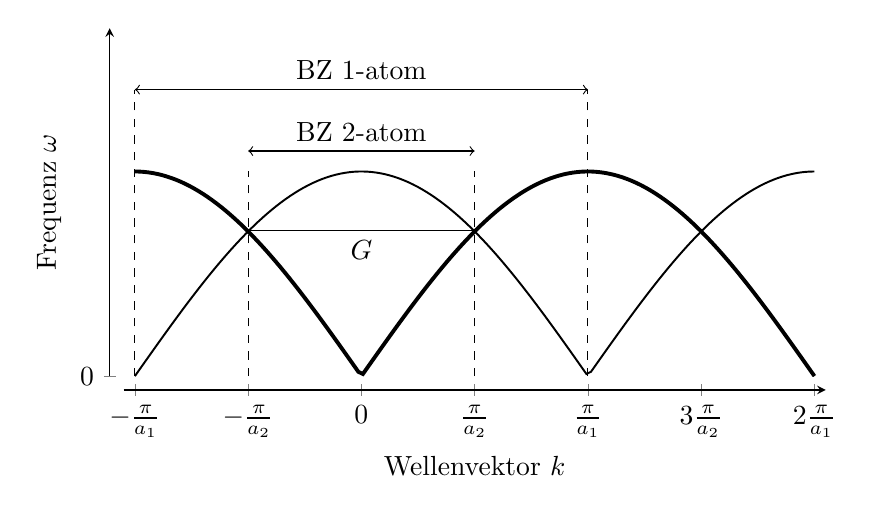
\begin{tikzpicture}[
declare function={ 
   m1 = 1;
   m2 = 1;
   mu = (m1 * m2) / (m1 + m2);
   omp(\x) = ( 1/mu ) + sqrt( (1 / mu^2) - (4 / (m1 * m2))  * sin(\x) ^2);
   omm(\x) = ( 1/mu ) - sqrt( (1 / mu^2) - (4 / (m1 * m2))  * sin(\x) ^2);   
      %omp(\x) =  1 + sin(x) ;
	  },
]

%\omega^2 =  \frac{c}{\mu}
%\pm c \sqrt{ \frac{1}{\mu^2} - \frac{4}{M_1 M_2}  \sin^2 \left( %\frac{1}{2}  \mathbf{k} \cdot \mathbf{a} \right) } 


%\useasboundingbox (0,0) rectangle (5,5);
%\draw (0,0) rectangle (5,5);

\begin{axis}[no markers, 
	samples=150,
    %      ymin=-0.3, ymax=1,
     xmin = -2.1, xmax = 4.1,
    ymin = 0, ymax = 1.7,
      %  axis y line=left,
       %    axis x line=bottom,
         xtick = {-2, -1, 0,1,2, 3, 4},
          xticklabels= {$-\frac{\pi}{a_1}$,$-\frac{\pi}{a_2}$, 0, $\frac{\pi}{a_2}$, $\frac{\pi}{a_1}$, $3 \frac{\pi}{a_2}$, $2 \frac{\pi}{a_1}$ },
ytick = {0},
            xlabel = {Wellenvektor $k$ },
        ylabel = {Frequenz $\omega$},    
        %x label style={at={(axis description cs:1, 0)},anchor=north east, yshift=-7pt},
    %y label style={at={(axis description cs: 0,1)},anchor=south east,  yshift=10pt},
           width= 10.5cm, height = 6cm,
  separate axis lines,
  axis x line=bottom,
  axis x line shift=5pt,
  %xlabel shift=10pt,
  axis y line=left,
  axis y line shift=5pt,
%  ylabel shift=10pt           
           ]
           
\addplot [domain=-2:4,  line width=1.4pt]    {abs(sin(x * 45) ) };
\addplot [domain=-2:4,  line width=0.7pt]    {abs(sin(x * 45 + 90) ) };
 
\draw[->] (-1, 0.71) -- node[below]{$G$} (1,0.71); 
 
\draw[dashed] (-1,0) -- (-1, 1);  
\draw[dashed] (1,0) -- (1, 1);  
\draw[<->] (-1, 1.1) --node[above]{BZ 2-atom}  (1, 1.1);
 
 \draw[dashed] (-2,0) -- (-2, 1.4);  
\draw[dashed] (2,0) -- (2, 1.4);  
\draw[<->] (-2, 1.4) --node[above]{BZ 1-atom}  (2, 1.4);


 
 
%\node[anchor = north] at (0.5, 0.5) {\footnotesize akustisch} ;
%\node[anchor = north] at (0.3, 1.75) {\footnotesize optisch} ;
 
 
 \end{axis}

\end{tikzpicture}